\documentclass[a4paper, 11pt, twocolumn]{article}

\usepackage[a4paper, total={6.24in, 8.5in}]{geometry}
\usepackage[utf8]{inputenc}
\usepackage{graphicx}
\usepackage{verbatim}
\usepackage{float}
\usepackage{array}
\usepackage{xfrac}
\usepackage{mathpazo}
\usepackage{amsmath}
\usepackage{bm}
\usepackage{multirow}
\usepackage{makecell}
\usepackage{multicol}
\usepackage{sectsty,textcase}
\usepackage{wrapfig,lipsum,booktabs}
\usepackage{enumitem}
\usepackage{hyperref}
\usepackage{makecell}
\usepackage{array}

\bibliographystyle{plain}
% \renewcommand{\thesubsection}{\alph{subsection})}
\renewcommand{\thesection}{\arabic{section}}
%\renewcommand{\baselinestretch}{1.02}

%\setlength\parindent{0pt}
\setlength{\columnsep}{15pt}
\newcommand{\myparagraph}[1]{\paragraph{#1}\mbox{}\\}

\title{FYS-STK3155/4155 Applied Data Analysis and Machine Learning - Project 2: Classification and Regression }

\author{Lotsberg, Bernhard Nornes \\ Nguyen, Anh-Nguyet Lise \and \url{https://github.com/liseanh/FYS-STK4155-project2/}}
\date{October - November 2019}
\begin{document}
\twocolumn[
  \begin{@twocolumnfalse}
    \maketitle
    \begin{abstract}
      blip blop opnion wrong
    \end{abstract}
  \end{@twocolumnfalse}
]

\section{Introduction}
Classification in statistical analysis is a useful tool, e.g. for predicting
outcomes of various situations or classifying and sorting large amounts of data.

The aim of this project is  to study classification and regression problems
through our own implementation of logistic regression and a multilayer perceptron
(MLP) in Python. The particular data set we will be studying for classification
has been used in a prior research paper by Yeh, I. C. and Che-hui Lien about
data mining techniques \cite{origarticle}, which we will compare some of our
results with.  The full data set can be downloaded from the \href{https://archive.ics.uci.edu/ml/datasets/default+of+credit+card+clients}{UCI Machine
Learning Repository} \cite{UCI}. The data set contains certain features of
credit card clients' default payment from a Taiwanese bank.
For the regression problem we will use the MLP to approximate Franke's function
and compare with results from a prior project where we used ordinary least
squares, ridge and lasso regression to approximate it. \cite{regpaper}.


\section{Learning methods}
\subsection{Logistic Regression (LR)}
Logistic regression (LR)  is a statistical model that can be used to predict a
binary dependent variable. It functions in a manner similar to linear regression
(hence the name), the difference being that the outputs are put through an
activation function. Usually this activation function is the Sigmoid function,
which for abinary case with logistic regression is defined as
\begin{equation}
p(y=1 | X, \bm{\beta}) = \frac{1}{1 + e^{-X \beta}} =\frac{e^{X \beta}}{e^{X \beta}+1}.
\label{sigmoid}
\end{equation}
Here $X$ is the design matrix, and $\beta$ is a vector containing the weights
assigned to each
feature in $X$. It is useful to use another cost function than the mean squared
error, as the output
from our logistic regression is defined as $\hat{y}=p(X)\in [0, 1]$, where we
say that outcome 0 is predicted if $\hat{y}< 0.5$ and outcome 1 else. The cost
function most commonly used in this case is called the cross entropy, and is
defined as
\begin{align}
\mathcal{C_\text{ LR}}(\bm{\beta}) =& -\sum_{i=0}^{n-1} \left[\  y_i\log p(y_i|x_i, \bm{\beta}) \right. \nonumber\\
 &\left.+ (1-y_i)\log(1-p(y_i|x_i,\bm{\beta})    \right]
\end{align}
We find the weights $\bm{\beta}$ by solving $\text{argmin}_{\bm{\beta}}$. Like with
LASSO regression which we used in our previous project, this has no analytical
solution and must be estimated using gradient descent \cite{regpaper}. This
along with its stochastic sibling is described in section \ref{SGD}.

In this project we will use LR on the Taiwanese credit card data to try to predict
default ($y=1$) or non-default ($y=0$) payment and evaluate the model's predictive
accuracy in this particular classification problem.

\subsection{Neural Networks (NN)}

An artificial neural network (NN) is a computational model consisting of
interconnected nodes. The interconnected nodes aim to emulate a simplified
biological neural network and neuronal firing in a brain , and are therefore
also commonly referred to as neurons.  The node performs a weighted sum of its
inputs that is subsequently passed through a mathematical function to determine
its output. This mathematical function is called an activation function $f(z)$,
and should emulate neuronal firing.

There is a wide variety of different neural networks. Commonly, they consist of
layers of nodes separated into the input layer and output layer, and may also
contain one or more in-between layers called hidden layers. One such NN is the
multilayer perceptron (MLP), which is what we will be using in this project for
both classification and regression.
\subsection{Multilayer perceptron (MLP)}

\subsubsection{Feed-forward  }
The multilayer perceptron is a feed-forward neural network (FFNN), which means
that the information flows forward only, starting from the input layer and to
the output layer. Additionally, if each of the nodes in a layer is connected to
all of the nodes in the succeeding layer, the network is fully connected. The
inputs of the node are the weighted outputs of the nodes from the preceding
layer, in addition to a bias term that can control whether or not the neuron
fires if all the inputs are zero \cite{ML_algo}. The weighted sum of the inputs
of each node is called the activation.

\subsubsection*{Mathematical algorithm} \myparagraph{Input layer}
Starting with the input layer, which is the first layer in the MLP, the
activation is calculated using the input coordinates $x_j$,
\begin{equation}
z_i^1 = \sum^{M_1}_{j=1}w_{ij}^1x_j + b_i^1,
\end{equation}
where the superscript 1 indicates the first layer, $M_1$ is the number of inputs
to the $i$th node in the first layer, $b_i$ is the bias and $w_{ij}$ represents
the weights.

The output of the nodes in the input layer is determined by the activation
function $f(z)$,
\begin{equation}
f(z_i^1) = f \left( \sum^{M_1}_{j=1}w_{ij}^1x_j + b_i^1 \right)
\end{equation}
\myparagraph{Hidden layers and output layer}
Similarly for the subsequent layers; the hidden layers and the output layer, the
activation of the $j$th neuron of layer $l$ is defined as
\begin{equation}
z_j^l = \sum_{i=1}^{M_{l-1}} w_{ij}^la_j^{l-1} + b_j^l,
\end{equation}
where $b_j^l$ and $w_{ij}^l$ are the biases and weights at layer $l$, ${M_{l-1}}$
is the number of nodes at layer $l-1$ and $a_j^{l-1}=f(z_j^{l-1}) $.
The output of each node is then decided by passing the activation through the
activation function,
\begin{equation}
 f(z_j^l) =f \left(     \sum_{i=1}^{M_{l-1}} w_{ij}^la_j^{l-1} + b_j^l \right)
\end{equation}
This is nearly identical to the method for the input layer, except that the
inputs of these layers are the outputs from the previous layer.

\subsubsection{Backpropagation} \label{subsub:backpropagation}
In order for the NN to learn, the weights and biases are initialized with values
that we will discuss shortly. The weights and biases are then optimalized to
minimize the cost function through a process called backpropagation, where we
iterate backwards from the last layer to the first hidden layer. Another feed-forward process is initiated  from the input layer to the output layer with the new
biases and weights. If the cost function is not yet sufficiently minimized, then
backpropagation is performed again. This process is repeated until the cost
function is optimalized.

\myparagraph{Mathematical algorithm}
To calculate the optimal biases and weights for the problem, we initialize the
gradients of the cost function $\mathcal{C}$ with respect to the  weights $W$
and biases $b$ at the output  layer $l=L$ 	and the output error $\delta_L$ as
\begin{flalign}
&\frac{\partial  \mathcal{C}}{\partial w^L_{jk}} = \delta^L_j a_k^{L-1},
\label{eq:dC/dw_L}\\
&\frac{\partial  \mathcal{C}}{\partial b^L_j} = \delta^L_j,\\
&\delta_j^L= f'(z_j^L)\frac{\partial \mathcal{C}}{\partial a_j^L},
\label{eq:delta_j^L}
\end{flalign}
before propagating backwards through the hidden layers using the general equations
\begin{flalign}
&\frac{\partial  \mathcal{C}}{\partial w^l_{jk}} = \delta^l_j a_k^{l-1},
\label{eq:dC/dw_l} \\
&\frac{\partial  \mathcal{C}}{\partial b^l_j} = \delta^l_j,\\
&\delta_j^l= \sum_k \delta_k^{l+1}w_{kj}^{l+1}f'(z_j^l). \label{eq:delta_j^ l}
\end{flalign}
The full derivation of these equations can be found in \textit{Neural networks,
from the simple perceptron to deep learning} by Morthen Hjorth-Jensen \cite{morten_NN}.

\subsubsection{Choosing activation function}
There are certain properties that an activation function $f(z)$ should possess
\cite{ML_algo}:
\begin{enumerate}
\item $f(z)$ should be differentiable (continuous). \label{item:differentiable_f}
\item $f(z)$ should be non-constant and  reach saturation at both ends of the range.
\item $f(z)$ should change quickly between the saturation values  at the middle
of the range.
\end{enumerate}
It is clear  from Equation (\ref{eq:delta_j^ l}) in the backpropagation algorithm
that the activation function $f(z)$ should be differentiable, while the remaining
properties are mainly related to the emulation of firing of neurons in a brain.

There are several functions that meet these requirements. Historically, the
sigmoid function has been a popular choice of activation function until recently.
To compare our results with the original paper from 2009 by I-Cheng Yeh and
Che-hui Lien \cite{origarticle}, we have chosen to use the sigmoid function in
our implementation of the MLP, as it is likely the same function they used. The
function is given by
\begin{equation}
	f(z) = \frac{1}{1+e^{-z}}\ .
\end{equation}
Its gradient is given by
\begin{equation}
	\label{eq:df/dz}
	\frac{\partial f}{\partial z} = \frac{e^{-z}}{(1+e^{-z})^2}.
\end{equation}
However, there are cases where we do not want a sigmoidal output activation
function, such as for regression problems where the outputs should be from a
continuous range instead of binary. Instead of a sigmoidal activation function
for the regression case at output layer $l=L$, we implement a linear activation
function, such that
\begin{equation}
f(z_j^L)=z_j^L= \sum_{i=1}^{M_{L-1}} w_{ij}^L a_j^{L-1} + b_j^L.
\end{equation}
For our binary classification case, we keep the sigmoid function as the output
activation function.
\subsubsection{Choosing cost function}
Looking at the equations for backpropagation, it is clear that the chosen cost
function $\mathcal{C}$ should be differentiable as well.
Additionally, the cost function should be chosen with the desired functionality
in mind, i.e. the cost functions for regression and classification should be different.

For the classification part of this project we have chosen to use the logistic
loss as cost function, which is the negative log-likelihood,
\begin{align}
\mathcal{C_\text{ NN}^\text{ C}}&(\bm{W}, \bm{b}) = -\sum_{i=0}^{n-1}
\left[\  a_i^l\log p\left(a_i^l|z_i^l,\ \bm{ W,\ b} \right) \right.  \\
&   \left. + (1-a_i^l)\log \left(1-p(a_i^l|z_i^l,\ \bm{ W,\ b} )\right) \right],
\nonumber
\end{align}
with $a_i^l=f(z_i^l)$ as before. The gradient at the last layer is
\begin{align}
\frac{ \partial C_\text{ NN}^\text{ C}}  {\partial a_i^L} =
a_i^L-t_i, \label{eq:dC/da_NN^C}
\end{align}
where $t_i$ is the target.\\

For the regression part we will use the cost function
\begin{equation}
\mathcal{C}_\text{ NN}^\text{ R} = \frac{1}{2}\sum_{i=0}^{n-1}(t_i-a_i^l)^2.
\end{equation}
The gradient in the last layer is given by
\begin{equation}
	\frac{\partial \mathcal{C}_\text{ NN}^\text{ R}}{\partial a_i^L}=t_i -a_i^L\ .
	\label{eq:dC/da_NN^R}
\end{equation}

The gradients in Equation (\ref{eq:dC/da_NN^C}) and (\ref{eq:dC/da_NN^R}) can then be inserted into Equation (\ref{eq:delta_j^ l}) in the backpropagation algorithm.
\subsubsection{Initialising  the weights and biases}
The biases can be initialized to zero, but we have chosen an initial value of 0.01
to ensure that all of the neurons have some initial output. Initializing the
weights to zero, however, will result in all neurons outputting the same value.
Instead, the  weights are initialized with values drawn from a uniform distribution
such that $w_{kj}\in (-1/\sqrt{n}, \ 1/\sqrt{n})$, where $n$ is the amount of
nodes in the input layer,  to ensure uniform learning \cite{ML_algo}.

\subsubsection{Regularization}
As neural networks often have large amounts of parameters, they are considered
very high variance low bias estimators. This means they are very prone to
overfitting. To counteract this, we introduce regularization using the $L_2$
penalty on the weights similarily to Ridge regression. Mathematically, this means
adding the regularized cost function becomes
\begin{equation}
  \mathcal{C}_{\text{Regularized}} = \mathcal{C}_\text{ NN}^{C/R} + \lambda ||\bm{W}||_2^2
  \label{Regularized cost}
\end{equation}
and its derivative becomes
\begin{equation}
  \frac{ \partial C}  {\partial \bm{W}}_\text{Regularized}
  = \frac{ \partial C_\text{ NN}^\text{ C/R}}  {\partial \bm{W}} + \lambda \bm{W}.
\end{equation}
Here $\lambda$ is a hyperparameter we need to tune.

\subsection{Stochastic Gradient Descent (SGD)}
\label{SGD}
It is clear that in order to find the best possible fit, we need to optimize the
cost function $\mathcal{C}$ by finding its minimum. A common method to achieve
this is the gradient descent (GD) method, in which the parameters $\theta$ are
iteratively adjusted in the direction of the largest negative value of the
gradient for a given number of iterations or until it reaches a given tolerance.
Mathematically, this is expressed as
\begin{equation}
\theta_{i+1} = \theta_i -\eta \nabla \mathcal{C}(\theta_i),
\end{equation}
where $\eta$ is the learning rate, which is a hyperparameter that controls the
step length and by extension the convergence time. For smaller values of $\eta$,
the method will take longer to converge or might not converge at all within a
desired time frame. For larger values of $\eta$, the method might be unstable or
pass the minimum altogether and diverge. The parameter $\theta$ is $\beta$ in
the LR case, and the weights $W$ and biases $b$ in the MLP case.

However, calculating the gradient on the entire data set can be computationally
expensive and inefficient for large amounts of data. Additionally, there is a high
possibility of a local minimum being misinterpreted as a global minimum by the
algorithm. To alleviate these problems, we can use stochastic gradient descent
(SGD) with minibatches.  A minibatch is a subset of the data, on which we can
perform GD. By using stochasticity to perform gradient descent on randomly chosen
minibatches of size $M$, we have a more efficient way to approximate the gradient
of the total data set as it might not need to use the entire set. Additionally,
the stochasticity reduces the possibility of getting stuck in a local minimum.

\subsection{Choosing hyperparameters}
Hyperparameters have to be found via trial and error. 

\section{Data}
\subsection{Classification - Credit card client data}
For the classification part of this project,  we are using credit card payment
data from a Taiwanese bank downloaded from the \href{https://archive.ics.uci.edu/ml/datasets/default+of+credit+card+clients}{UCI Machine Learning Repository}. The
response variable is a binary variable of default payment with Yes = 1, No = 0.
The original data set consists of 30 000 observations, with X amount of
observations with default payments. There are 23 explanatory variables, cited
from the original paper they are described as \cite{origarticle}:
\begin{itemize}[leftmargin=5mm, itemsep=0pt,  parsep=1pt]
 \item X1: Amount of the given credit (NT dollar): it includes both the individual consumer credit and his/her family (supplementary) credit.
\item X2: Gender (1 = male; 2 = female).
\item X3: Education (1 = graduate school; 2 = university; 3 = high school; 4 = others).
\item X4: Marital status (1 = married; 2 = single; 3 = others).
\item X5: Age (year).
\item X6 - X11: History of past payment. We tracked the past monthly payment
records (from April to September, 2005) as follows: X6 = the repayment status in
September, 2005; X7 = the repayment status in August, 2005; . . .;X11 = the
repayment status in April, 2005. The measurement scale for the repayment status
is: -1 = pay duly; 1 = payment delay for one month; 2 = payment delay for two
months; . . .; 8 = payment delay for eight months; 9 = payment delay for nine
months and above.
\item X12-X17: Amount of bill statement (NT dollar). X12 = amount of bill
statement in September, 2005; X13 = amount of bill statement in August, 2005;
. . .; X17 = amount of bill statement in April, 2005.
\item X18-X23: Amount of previous payment (NT dollar). X18 = amount paid in
September, 2005; X19 = amount paid in August, 2005; . . .; X23 = amount paid in
April, 2005.
\end{itemize}

\subsection{Regression - Franke's function}
For the regression part part of this project we will be performing regression
analysis on Franke's function $g(x,y)$ with added Gaussian noise $\bm{\varepsilon}
\sim N(0,\  \sigma^2) $. Franke's function is given by
\begin{align}
g(x,y) &= \frac{3}{4}\exp{\left(-\frac{(9x-2)^2}{4}   - \frac{(9y-2)^2}{4}\right)} \nonumber\\
 &+\frac{3}{4}\exp{\left(-\frac{(9x+1)^2}{49}- \frac{(9y+1)}{10}\right)} \nonumber\\
 &+\frac{1}{2}\exp{\left(-\frac{(9x-7)^2}{4} - \frac{(9y-3)^2}{4}\right)} \nonumber\\
 &-\frac{1}{5}\exp{\left(-(9x-4)^2 - (9y-7)^2\right) }  \label{eq:Franke}
\end{align} and is defined on $x,\ y \in [0,1]$. The data we are fitting is
given by
$$G(\bm{x}, \bm{y}) = g(\bm{x}, \bm{y}) + \bm{\varepsilon},$$
where $\bm{x},\ \bm{y}$ are vectors of uniformly spaced values from 0 and 1 of
length $n_x$ and $n_y$ respectively. To directly compare with our previous
project, \textit{Project 1: Regression analysis and resampling methods}
\cite{regpaper}, we choose to generate and analyze the data sets \texttt{franke0},
\texttt{franke1}, \texttt{franke2} as configured in Table \ref{tab:franke_dataset}.
To generate the points, we grid over $n_x$ points in $x$-direction and $n_y$ points
in $y$-direction.
\textbf{WE NEED TO TALK MORE ABOUT OUR PREVIOUS ANALYSIS AND WHAT KIND OF METHODS
AND PARAMETERS WE USED }

\begin{table}[H]
	\caption{Table of the configurations for our generated data sets using
	Franke's function given in Equation (\ref{eq:Franke}) with added noise $\bm
	{\varepsilon} \sim N(0,\  \sigma^2) $. $n_x$ and $n_y$  indicate the number
	of points used to produce the grid in their respective directions. }
	\label{tab:franke_dataset}
	\resizebox{\columnwidth}{!}{
	\begin{tabular}{|l|l|l|l|c|} \hline
	Data set &  Data points	&$n_x$ & $n_y$ & $\sigma$ \\ \hline
	\texttt{franke0} & 400 & 20 & 20 & 1.0\\ \hline
	\texttt{franke1	} & 400 & 20 & 20 & 0.10\\ \hline
	\texttt{franke2} & 40 000& 200 & 200 & 0.10 \\ \hline
	\end{tabular}
	}
\end{table}

\section{Model evaluation}
\subsection{Regression}
To evaluate the performance of our regression model, we consider the $R^2$ score,
given by
\begin{equation}
	R^2(\bm{y}, \bm{\hat{y}}) = 1 - \frac{\sum_{i=0}^{n - 1} (y_i -
	\hat{y}_i)^2}{\sum_{i=0}^{n - 1} (y_i - \bar{y})^2},
    \label{eq:R2}
\end{equation}
where $\bm{y}$ is the given data, $\bm{\hat{y}}$ is the model and ${\bar{y}}$ is
the mean value of $\bm{y}$.
\subsection{Classification}
To evaluate the performance of our classification model, we consider the accuracy
score, given by
\begin{equation}
\label{eq:accuracy}
\text{accuracy}=\frac{\sum_{i=1}^nI(t_i=y_i)}{n},
\end{equation}
where $t_i$ is the target, $y_i$ is the model output, $n$ is the number of
samples and $I$ is the indicator function,
\[
I = \begin{cases}
1, & t_i = y_i\\
0, & t_i \neq y_i
\end{cases} .
\]

\section{Results}

\begin{figure}[H]
	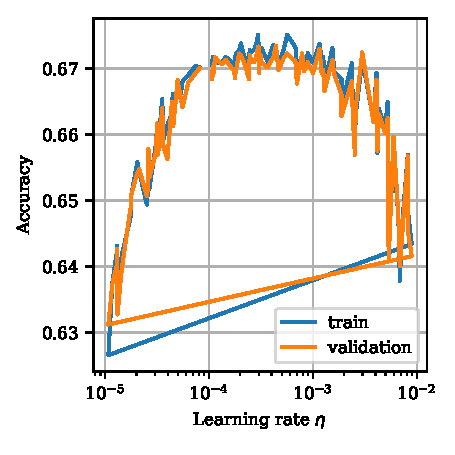
\includegraphics[scale=1]{figures/logreg_learning_rate_accuracy.pdf}
	\caption{Accuracy score of validation set of the credit card data using the
	logistic regression classifier. The values of the shrinkage parameter
	$\lambda$ were chosen using randomized search.}
	\label{fig:logreg_eta_accuracy}
\end{figure}


\begin{table}[H]
	\caption{Table of error rates and area ratios for classification of the
	credit card data using logistic regression (LR) and the multilayer
	perceptron (MLP) neural network (NN).}
	\label{tab:area_ratios}
	\resizebox{\columnwidth}{!}{
 	\begin{tabular}{|l|l|l|l|}
    \hline
 	   Method & \makecell[l]{Error \\rate} & \makecell[l]{Area ratio \\default} & \makecell[l]{Area ratio \\non-default} \\ 			\hline
    		LR & 0.31  & 0.43 & 0.12 \\ \hline
    		NN & 0.22  & 0.55 & 0.16 \\ \hline
    	\end{tabular}
	}
\end{table}

\begin{table}[H]
	\caption{Table of R2 scores for our neural network (NN) regression models on
	the three Franke data sets and the ordinary least squares (OLS) model from our
	previous study \cite{regpaper}. }
	\label{tab:R2_scores}
	\resizebox{\columnwidth}{!}{
 	\begin{tabular}{|l|r|r|r|r|}
    \hline
 	     {} &$R^2$  & \texttt{franke0} & \texttt{franke1} &	\texttt{franke2} \\	\hline
    	 \multirow{2}{*}{NN}  &Train   & 0.0052  & 0.59 & 0.84 \\ \cline{2-5}
    		 				  &Test    & - 0.057 & 0.59 & 0.83 \\ \hline
    \multirow{2}{*}{OLS}      &Train   & 0.024   & 0.87	& N/A \\ \cline{2-5}
    		 				  & Test   & - 0.040 & 0.82 & N/A\\ \hline
    	\end{tabular}
	}
\end{table}

\begin{table}[H]
  \caption{Table of the best hyperparameters values for shrinkage $\lambda$ and
  learning rate $\eta$ for the logistic regression (LR) and neural network (NN)
  models. The parameters were found using 5-fold cross validation. The minibatch
  size was kept constant at $M=200$. }
  \label{tab:hyperparameters}
{\setlength{\extrarowheight}{2pt}
  	\resizebox{\columnwidth}{!}{
  \begin{tabular}{|l|l|l|}
    \hline
    Model & Shrinkage $\lambda$ & Learning rate $\eta$ \\ \hline
    LR credit data & N/A & $4.4 \cdot 10^{-4}$ \\ \hline
    NN credit data & $6.9 \cdot 10^{-7}$ & $7.7 \cdot 10^{-2}$ \\ \hline
    NN \texttt{franke0} & $4.1\cdot 10^{-6}$ & $9.1\cdot 10^{-5}$ \\ \hline
    NN \texttt{franke1} & $6.4\cdot 10^{-8}$ & $1.5 \cdot 10^{-4}$\\ \hline
    NN \texttt{franke2} & $3.6\cdot 10^{-10}$ & $3.7 \cdot 10^{-4}$\\ \hline
  \end{tabular}
  }}
\end{table}

\begin{figure}[H]
	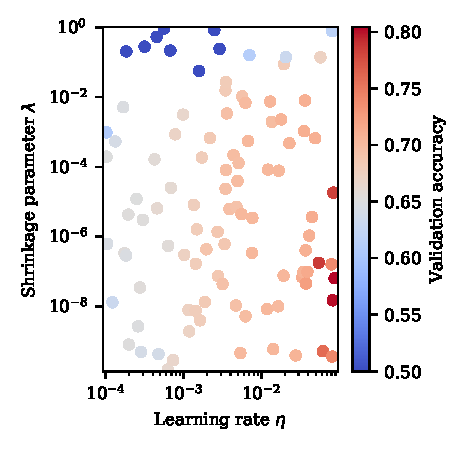
\includegraphics[scale=1]{figures/nn_learning_rate_lambda_accuracy_credit.pdf}
	\caption{Accuracy score of validation set of the credit card data using the
	multilayer perceptron classifier. The values of the shrinkage parameter
	$\lambda$ and the learning rate $\eta$ were chosen using randomized search.}
	\label{fig:nn_eta_lambda_credit_accuracy}
\end{figure}



\begin{figure}[H]
	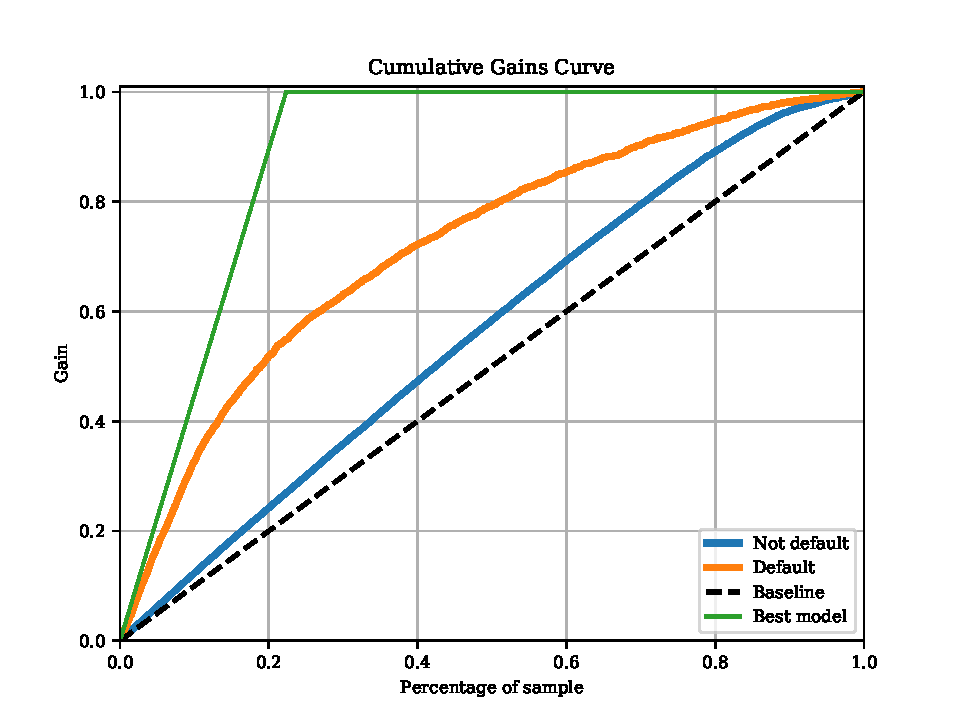
\includegraphics[scale=1]{figures/cumulative_gain_NN.pdf}
	\caption{idk yet}
	\label{fig:nn_gain}
\end{figure}

\begin{figure}[H]
	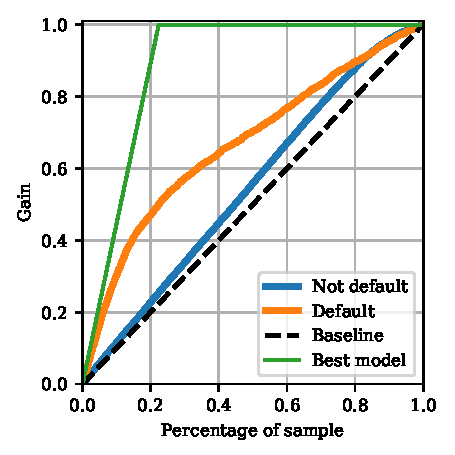
\includegraphics[scale=1]{figures/cumulative_gain_logreg.pdf}
	\caption{idk yet}
	\label{fig:logreg_gain}
\end{figure}


\begin{figure}[H]
	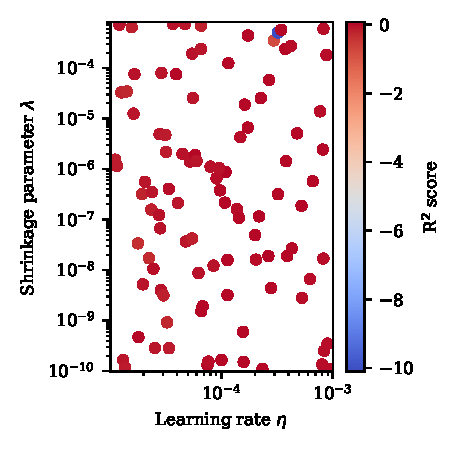
\includegraphics[scale=1]{{figures/nn_learning_rate_lambda_r2_franke_20_20_1.0}.pdf}
	\caption{$R^2$ score of validation set of the Franke function data set with
	400 total points $n_x=n_y=20,\ \sigma=1.0$ using the multilayer perceptron
	regressor. The values of the shrinkage parameter $\lambda$ and the learning
	rate $\eta$ were chosen using randomized grid search.}
	\label{fig:nn_eta_lambda_r2_400_1.0}
\end{figure}


\begin{figure}[H]
	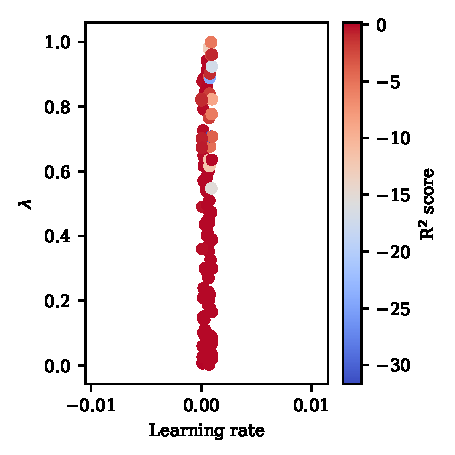
\includegraphics[scale=1]{{figures/nn_learning_rate_lambda_r2_franke_20_20_0.1}.pdf}
	\caption{$R^2$ score of validation set of the Franke function data set with
	400 total points, $n_x=n_y=20,\ \sigma=0.1 $ using the multilayer perceptron
	regressor. The values of the shrinkage parameter $\lambda$ and the learning
	rate $\eta$ were chosen using randomized grid search.}
	\label{fig:nn_eta_lambda_r2_400_0.1}
\end{figure}


\begin{figure}[H]
	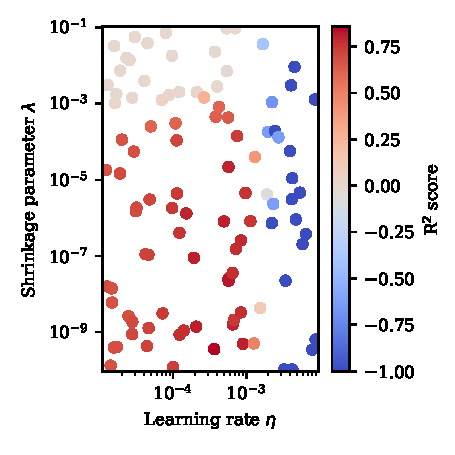
\includegraphics[scale=1]{{figures/nn_learning_rate_lambda_r2_franke_200_200_0.1}.pdf}
	\caption{$R^2$ score of validation set of Franke function data with 40 000
	total points, $n_x=n_y=200,\ \sigma=0.1 $ using the multilayer perceptron
	regressor. The values of the shrinkage parameter $\lambda$ and the learning
	rate $\eta$ were chosen using randomized grid search.}
	\label{fig:nn_eta_lambda_r2_40000_0.1}
\end{figure}

\begin{figure*}
	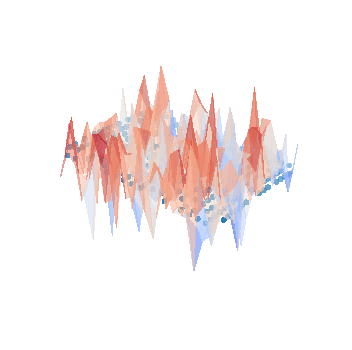
\includegraphics[width=\columnwidth]{{figures/3dplot_train_20_20_1.0}.pdf}
	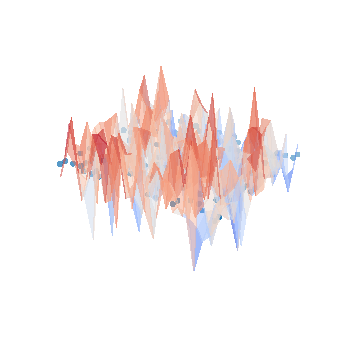
\includegraphics[width=\columnwidth]{{figures/3dplot_test_20_20_1.0}.pdf}
	\caption{3D plot of the Franke function with added noise $\sim\mathcal{N}(0,
	\sigma^2)$ with $\sigma=1.0$. The dotted markers represent the regression
	model found using MLP. The left plot shows the model fitted on the training
	set, the right shows the model fitted on the test set. The total data set
	consist of 400 points, using two thirds $(\sfrac{2}{3})$ as the training set
	and the remaining points $(\sfrac{1}{3})$ as the test set. }
	\label{fig:3dplot_400_1.0}
\end{figure*}

\begin{figure*}
	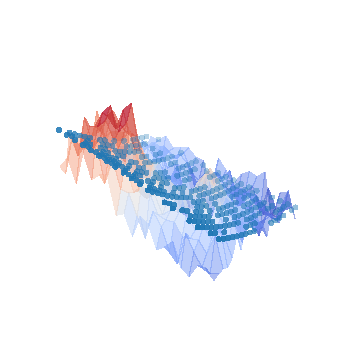
\includegraphics[width=\columnwidth]{{figures/3dplot_train_20_20_0.1}.pdf}
	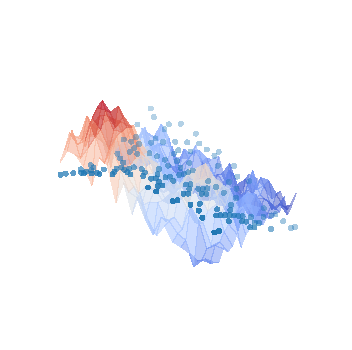
\includegraphics[width=\columnwidth]{{figures/3dplot_test_20_20_0.1}.pdf}
	\caption{3D plot of the Franke function with added noise $\sim\mathcal{N}(0,
	\sigma^2)$ with $\sigma=0.1$. The dotted markers represent the regression
	model found using MLP. The left plot shows the model fitted on the
	training set, the right shows the model fitted on the test set. The total
	data set consist of 400 points, using two thirds $(\sfrac{2}{3})$ as the
	training set and the remaining points $(\sfrac{1}{3})$ as the test set. }
	\label{fig:3dplot_400_0.1}
\end{figure*}

\begin{figure*}
	\includegraphics[width=\columnwidth]{{figures/3dplot_train_200_200_0.1}.pdf}
	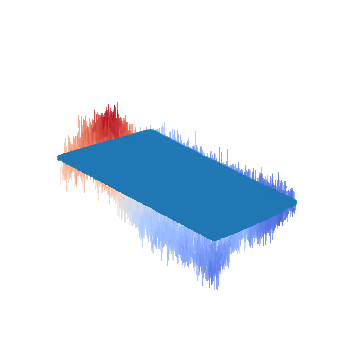
\includegraphics[width=\columnwidth]{{figures/3dplot_test_200_200_0.1}.pdf}
	\caption{3D plot of the Franke function with added noise $\sim\mathcal{N}(0,
	\sigma^2)$ with $\sigma=0.1$. The dotted markers represent the regression
	model found using MLP. The left shows the model fitted on the training set,
	the right shows the model fitted on the test set. The total data set consist
	of 40 000 points, using two thirds $(\sfrac{2}{3})$ as the training set and
	the remaining points $(\sfrac{1}{3})$ as the test set. }
	\label{fig:3dplot_40000_0.1}
\end{figure*}

\section{Discussion}
fill
\section{Conclusion}
fill
%\bibliographystyle{iEEEtran}
\bibliography{references}



\end{document}
